\documentclass[pdftex,12pt,a4paper]{report}
\usepackage[utf8]{inputenc}
\usepackage[portuguese]{babel}
\usepackage{graphicx}
\usepackage[T1]{fontenc}
\usepackage{times}
\usepackage{float}
\usepackage{geometry}
\geometry{margin=1in}
\usepackage[fleqn]{amsmath}
\usepackage{MnSymbol}  
\usepackage{hyperref}

\newcommand{\RomanNumeralCaps}[1]
    {\MakeUppercase{\romannumeral #1}}

\usepackage{listings}
\usepackage{color} 
 
\definecolor{codegreen}{rgb}{0,0.6,0}
\definecolor{codegray}{rgb}{0.5,0.5,0.5}
\definecolor{codepurple}{rgb}{0.58,0,0.82}
\definecolor{backcolour}{rgb}{0.95,0.95,0.92}
 
\lstdefinestyle{mystyle}{
    backgroundcolor=\color{backcolour},   
    commentstyle=\color{codegreen},
    keywordstyle=\color{magenta},
    numberstyle=\tiny\color{codegray},
    stringstyle=\color{codepurple},
    basicstyle=\footnotesize,
    breakatwhitespace=false,         
    breaklines=true,                 
    captionpos=b,                    
    keepspaces=true,                 
    numbers=left,                    
    numbersep=5pt,                  
    showspaces=false,                
    showstringspaces=false,
    showtabs=false,                  
    tabsize=2
}
 
\lstset{style=mystyle}

\usepackage{titlesec}
\titleformat{\chapter}% reformat chapter headings
     [hang]% like section, with number on same line
     {\Huge\bfseries}% formatting applied to whole
     {\thechapter}% Chapter number
     {0.5em}% space between # and title
     {}% formatting applied just to title 

\begin{document}
\begin{titlepage}
	\centering
	
\includegraphics[width=0.4\linewidth]{images/logo-ee.png}\\[4ex]
	{\scshape\LARGE Universidade do Minho \\ MIEI\par}
	\vspace{1cm}
    	{\scshape\Large Gestão de Processo de Software\par}
	\vspace{1.5cm}
	{\LARGE\bfseries
		Análise estática de normas de codificação\par }
	\vspace{1cm}
	
	\vfill 
	
    \textbf{Grupo 6:}\par
    José Pereira   -   a82880  \par
    Luís Braga     -   a82088  \par
	Luís Cunha     -   a83099\par
    Luís Martins   -   a82298\par
    Ricardo Petronilho - a81744   \par
	
	\vfill
	
	%--- Fim Capa ---%
	{\large Braga, Portugal\par \today\par}
\end{titlepage}
\newpage

\tableofcontents
\chapter{Introdução}

\hspace{5mm} No âmbito da unidade curricular de Gestão de Processo de Software, pertencente ao perfil de Engenharia de Software do 4ºano do Mestrado Integrado em Engenharia Informática, foi proposto aos alunos que construíssem um programa com o intuito de encontrar \textit{code smell's} e que, desta forma, pusessem à prova as boas práticas das linguagens orientadas aos objetos. Um \textit{code smell} é uma característica no código fonte de um determinado programa, que poderá servir de indicador para problemas mais graves. Portanto, pode-se assim compreender o interesse de desenvolver e de enveredar por este projecto.
\par O trabalho proposto indica que este projecto seja desenvolvido em C#. Contudo, foi permitido que viesse a ser realizado na linguagem de programação Java.
\par O desenvolvimento deste projecto é compreendido por duas partes distintas. A primeira consiste num levantamento de \textit{code smells} e de bons costumes de programação na área de programação orientada aos objectos da linguagem Java. A segunda consiste na construção de um programa ("tool") que identifique/recolha esses indicadores.


\chapter{Normas de Codificação}

\hspace{5mm} Ao longo deste capítulo descrevem-se os \textit{code smells} e outras boas práticas de programação que o grupo de trabalho considerou relevantes e seleccionou para a implementação.

\section{Code Smells}

\hspace{5mm} \textit{Code Smells} são características e particularidades encontradas no código de um determinado programa. Estas características podem ser indicadores ou sinais de que a implementação de um programa já possui ou poderá vir a apresentar problemas. Estes problemas encontram-se muitas vezes camuflados e não comprometem o correcto funcionamento do programa. Contudo, põem em risco o ciclo de vida do programa, pois, complicam, por vezes ao ponto de ter de se recomeçar do início o desenvolvimento, a evolução do programa, a sua manutenibilidade e a capacidade de outros perceberem o que foi feito.

\subsection{Bloaters}
\hspace{5mm} \textit{Bloaters} como o nome indica são porções de código, métodos ou classes que possuem proporções excessivas e que, consequentemente, se tornaram quase impossíveis de modificar, utilizar ou perceber.

\subsubsection{Long Method}
\hspace{5mm} Um \textit{smell} do tipo \textit{bloater} que foi seleccionado para desenvolver foi o \textit{long method}. Este "mau cheiro" traduz-se num método que contém demasiadas linhas de código. Este simples facto pode ser indicador que este mecanismo poderá ter sobre si demasiada responsabilidade, o que compromete a sua reutilização e a capacidade de se alterar no futuro.


\subsubsection{Large Class}
\hspace{5mm} De forma semelhante ao \textit{long method} a \textit{large class} é um classe que também é excessivamente grande e que possui demasiada responsabilidade. Normalmente a de eliminar este \textit{smell} é dividir esta classe em outras mais pequenas.


%%\section{Object-Orientation Abusers}

%%\section{Change Preventers}

\subsection{Dispensables}

\hspace{5mm} Um \textit{dispensable} é um tipo de \textit{bad smell} que consiste em alguma coisa que seja desnecessária e que não tenha sentido como, por exemplo, comentários, código duplicado, classes que têm poucas responsabilidades ou até nenhuma, classes que apenas guardam variáveis, mas não existe nenhuma lógica sobre esses dados, código que não é utilizado ou até funcionalidades que são feitas a pensar no futuro, mas que não utilizadas no presente. Todas estas situações fariam com que o código ficasse mais limpo, mais eficiente e mais fácil de compreender se fossem eliminadas.

\subsubsection{Comments}

\hspace{5mm} Os comentários podem parecer muitas vezes inofensivos e até facilitadores na percepção do trabalho que foi feito. Contudo, se retirarmos o comentário e, subitamente, o que está escrito se tornar muito mais difícil de compreender estamos perante um \textit{bad smell}. Isto significa que o código deve ser refeito e que os comentários servem de certa forma como uma máscara para certos problemas.

%%\section{Couplers}


\section{Bons Hábitos}

\hspace{5mm} Esta classe está reservada para situações que não são consideradas \textit{code smells}, mas que são consideradas bons costumes no momento de programação.

\subsection{toString(), equals(), clone()...}

\hspace{5mm} Uma classe deve ser robusta e apresentar alguma capacidade  de acomodar necessidades futuras. Para tal, existem algumas funções frequentes na programação orientada a objectos em Java que, apesar de nem sempre serem necessárias, quase sempre são implementadas de forma a tornar a classe mais completa e integra. Tais métodos podem ser, os diferentes tipos de construtor, como \textit{toString()}, o método \textit{clone()}, entre outros.

\subsection{Usar Variáveis Privadas}

\hspace{5mm} Numa classe, as variáveis de instância devem ser privadas. Isto deve ser visto um bom costume de programação, pois, comummente, a utilização de variáveis públicas está associada com a utilização directa das mesmas por outras classes. O que já é classificado como um \textit{bad smell} designado como \textit{Inappropriate Intimacy}.

\subsection{Nome da classe começada com letra maiúscula}

\hspace{5mm} O nome da classe deve ser iniciado com uma letra maiúscula, sendo uma boa prática também colocar o nome de uma variável de instância com letra minúscula, podendo assim ser mais fácil de distinguir classes de variáveis de instância, etc. De referir que também é identificado se o nome da classe possuí o mesmo nome que o nome do ficheiro associado à classe.

\subsection{Utilizar Interfaces Genéricas}

\hspace{5mm} Acoplamento e dependência excessiva são características dispensáveis no código e que têm de ser resolvidos o mais cedo possível, pois, corre-se o risco de inconvenientes futuros. Para atenuar este problema, poder-se-ão adoptar certas medidas como a utilização de interfaces genéricas. Isto é, devem-se utilizar interfaces como \textit{List} e \textit{Set} em vez de estruturas específicas, pois, desta forma, mudanças serão facilitadas no futuro.

\subsection{Utilização de Herança}

\hspace{5mm} Apesar de inúmeras vezes ser bem utilizado e estar perfeitamente enquadrado no contexto, o mecanismo de herança pode vir a ter consequências adversas. 
\par A utilização de herança implica que métodos e variáveis de instância sejam herdados pela classe que estende e isto causa dependências, que são por vezes, negligenciadas. Contudo, no futuro, se for necessário levar a cabo alterações na superclasse irão surgir problemas, pois o comportamento das subclasses pode alterar-se. Consequentemente, isto pode levar a que seja necessário alterar todas as subclasses. Caso isto aconteça a arquitectura deve ser repensada e a viabilidade da herança avaliada.

\subsection{Variáveis Insuficientemente Identificadas}

\hspace{5mm} No acto da programação muitas tarefas são executadas com uma atitude de "quick fix" e experimental. Além do mais, todo o código quando é criado é experimental, pois nunca se sabe se realmente funciona, e tenta-se construí-lo da forma mais rápida, tendo em mente alterações futuras que nem sempre acontecem, isto implica muitas vezes escrever de uma maneira resumida, sucinta e quase sempre apenas perceptível a quem o está a fazer. Ao não efectuar estas mudanças o que foi produzido pode ser dificilmente compreensível por alguém que de fora ou que venha a fazer parte da equipa no futuro ou até, eventualmente, por quem desenvolveu devido a esquecimento. Neste contexto, o colectivo de trabalho decidiu por recolher indicadores relativos a variáveis identificadas apenas por uma letra, que como se pode supor, são indícios de programação inacabada, por melhorar e de entraves à mudança futura.

\subsection{Ciclos Infinitos}

\hspace{5mm} Para um produto de software ser eficaz é impreterível que o mesmo acabe o processamento de qualquer que seja tarefa de que seja responsável. Caso contrário nenhum resultado surgirá, o programa é inútil  e todo o esforço realizado para a produzir o software é infrutífero. Um caso específico deste problema é a aplicação de ciclos \textit{while true} em que é necessário cumprir uma condição de forma a sair do ciclo. No entanto, nem sempre é fácil ou trivial verificar que o ciclo é quebrado. Assim, nesta ferramenta de análise estática, a presença destes casos é contabilizada como um smell.

\subsection{Utilização de Exceções}

\hspace{5mm} Os erros de software são normalmente causados por ação humana pelo que, é importante prevenir implementando capacidade de resposta em situação de erro de modo a evitar que todo o sistema falhe. Desta forma, o uso de exceções em métodos desenvolvidos é algo que deve ser sempre considerado de modo a captar possíveis falhas do sistema e antecipar o tratamento das mesmas. 
\par Assim, esta ferramenta está programando para detetar e expor todos os métodos que não implementem qualquer exceção, indicando que esses métodos são vulneráveis.

\subsection{Input e Output Genérico}

\hspace{5mm} A abstração no código é um factor de elevada importância o qual deve ser sempre tomado em conta, quando possível.
\par De facto, no input e output de métodos, devem ser sempre recebidas e retornadas as coleções mais genéricas possíveis de modo a seguir as boas práticas de programação. 
\par Deste modo, este sistema verifica todos os outputs e inputs de todos os métodos de modo a alertar quais os métodos que podiam tornar-se mais abstratos.


\chapter{Implementação}
\section{Base do programa}
\hspace{5mm} Inicialmente, começou-se por desenvolver a base do programa ("tool"), isto é, a leitura dos ficheiros com o código, para a estrutura/classe denominada \textbf{Ficheiro}. 

\hspace{5mm} A estrutura \textbf{Ficheiro}, contém a lista de linhas mesmo, bem como uma toda uma estrutura, para guardar de forma transiente os dados recolhidos durante a análise. 

\hspace{5mm} Após ter-se os ficheiros organizados em memória, poder-se-á proceder ao processamento dos mesmos, isto é, percorrer a lista de linhas presente na classe \textbf{Ficheiro}. A ideia consiste em processar cada linha e verificar na mesma as várias normas identificadas, e proceder às acções das mesmas em caso de existirem. As acções que provém da identificação de uma norma, vão desde guardar informação na estrutura, até acções mais complexas que envolvem mais do que uma linha, e dessa forma ter-se-á que activar algumas \textit{flags} de controlo, como por exemplo \textbf{insideMethod}, que indica que a análise do ficheiro encontra-se no momento no interior de um método, no entanto isto será abordado com mais detalhe adiante. Maior parte das identificações de normas tira partido do uso de expressões regulares que verificam os padrões das normas/code smells.

\section{Comentários no código}
\hspace{5mm} Os comentários tal como foi dito anteriormente são uma das normas seleccionadas para serem verificadas. Desta forma, o passo inicial foi identificar as várias formas de comentar em \textbf{Java}, das quais, o comentário numa linha, ou comentários de multi linha. 

O comentário numa única linha torna-se um caso simples de identificar, pois a expressão regular apenas são duas barras, no entanto, importa activar uma flag, para que os restantes testes de code smells sejam desactivados, pois não faz sentido processar quando estão em comentários. Ainda neste caso, guarda-se a linha onde ocorre este comentário para reportar.

De modo muito semelhante, o comentário multi linha, tem uma expressão regular idêntica, sendo uma barra e asterisco. Desta forma, tal como no comentário simples, necessita-se de guardar a linha onde começa o comentário, bem como activar uma flag para desactivar a identificação de outros code smells, enquanto não se chegar à linha onde o comentário termina. Após chegar à linha final do comentário, a flag é desactivada, e passa-se novamente a testar as outras normas.

\section{Variáveis Privadas}

\hspace{5mm} Neste projecto, o recurso a expressões regulares tornou-se prática recorrente e foi adoptada como a forma mais fácil e eficaz de captar os code smells ou a inesxistência destes. A captura de variáveis privadas não é excepção e fez-se uso da seguinte expressão regular com a finalidade de interceptar a ocorrência de declarações de variáveis privadas.
\par A seguinte \textit{String} contém a expressão regular para capturar estas ocorrências, que são tidas em conta como bons hábitos da programação, tanto que no html de output o utilizador é avisado se possui ou não variáveis privadas nas suas classes.

\vspace{0.5cm}

\begin{lstlisting}[language=Java]  
String variaveisPrivadasPadrao = "private[A-Za-z0-9 <>,\\[\\]]+[=;]";
\end{lstlisting}

\vspace{0.5cm}

\par Como se pode verificar, a expressão regular captura a palavra reservada "private" seguida caractéres possíveis em declarações, como letras, números, parêntesis rectos para declaração de arrays e os símbolos de maior e menor usados, por exemplo, na declaração de Maps. Acabando com a '=' caso seja feita uma atribuição imediatamente na declaração ou ';' caso seja o final da declaração.

\section{Uso de Herança}

\hspace{5mm} Para este caso específico não foi utilizada uma expressão regular, mas foi definida, oportunamente, aquando da verificação do nome da classe. Nesse momento é verificado se a declaração da classe contém em si a palavra \textit{extends}. Isto permite verificar se a classe estende uma outra classe e, se for o caso, o utilizador será avisado no output que tal acontece, pelo que deve ter cuidado com este mecanismo por motivos explicitados no capítulo anterior.

\section{Variáveis Insuficientemente Identificadas}

\hspace{5mm} No capítulo anterior são explicados vários bons hábitos de programação e os motivos pelos quais assim são considerados. Um deles são \textit{Variáveis Insuficientemente Identificadas}. Tendo em mente que  a recolha deste tipo de situações é a funcionalidade do programa, poder-se-á dizer que esta funcionalidade visa capturar declarações de variáveis que tenham como nome uma única letra. Para tal, dentro de todos os métodos recebidos como input é verificado se tal declaração acontece. Para o efeito, foi criada a expressão regular descrita a seguir, que é basilar na implementação desta funcionalidade.

\vspace{0.5cm}

\begin{lstlisting}[language=Java]  
String variaveisUmCarater = "(final)?[A-Za-z\\[\\]<>, ]+ +[A-Za-z] *[;=]";
\end{lstlisting}

\vspace{0.5cm}

\par De forma semelhante à captura de variáveis privadas faz-se a captura variáveis com apenas um carácter. Contudo, desta vez, isto é realizado no interior de métodos e têm de se ter em conta algumas coisas diferentes como, por exemplo, a possibilidade de atributos como final e como seria de esperar apenas uma letra.432

\section{Long Method}

\par De forma a verificar a existência deste smell é necessário contar o número de linhas de cada método. Para isso é necessário saber onde cada método começa pelo que se utilizou a seguinte expressão regular.

\begin{lstlisting}[language=Java]  
String nomeMetodoPadrao = "(public|protected|private|static)(\\ |\\t)+(?!class)[A-Za-z<>]+(\\ |\\t)+[A-Za-z]+(\\ |\\t)*(\\ |\\(.*\\{)";
\end{lstlisting}

\par Efectivamente, esta expressão regular generaliza a declaração de um método permitindo determinar se se está na sua presença. Desta forma guarda-se registo do inicio de um método.
\par Depois de se saber onde começa o método é agora necessário contar as linhas do mesmo até ao seu termino. Para descobrir onde um determinado método acaba é utilizada a diferença entre o número de chavetas de "abrir e fechar" de modo a que, quando essa diferença for zero, sabe-se então que o método terminou.

\section{Inexistência Exceções nos métodos}

\par Para se verificar se um método implementa ou não exceções é necessário analisar a sua declaração. Para isso utiliza-se a expressão regular mencionada no code smell longMethod de modo a filtrar as declarações dos métodos para posteriormente aplicar a seguinte expressão regular sobre essas declarações.

\begin{lstlisting}[language=Java]  
    final String excecaoPadrao ="throws";
\end{lstlisting}

\par De facto, esta expressão regular verifica se um dado método implementa algum tipo de exceção de modo a registar todos os métodos que não o façam.


\section{Retornar e receber objectos Genéricos}

\par Efectivamente, para verificar se um método recebe e retorna objectos o mais genéricos possíveis, de modo a promover a abstração do código, foi tomada uma abordagem em que se listaram todas as coleções de objectos menos abstratas, de modo a encontrar os métodos que as recebam ou retornem. De seguida, mais uma vez utilizou-se a expressão regular do code smell longMethod de modo a encontrar as declarações de todos os métodos para então aplicar a seguinte expressão regular a essas declarações:

\begin{lstlisting}[language=Java]  
String inputOutputPadrao = "(ArrayList|List|HashMap|Set|Queue|Dequeue|Map|ListIterator|SortedSet|SortedMap|HashSet|TreeSet|LinkedList|TreeMap|PriorityQueue)";
\end{lstlisting}

\par Caso a declaração de um determinado método contenha, quer no seu input ou output, algum dos objectos captados pela expressão regular, este será registado como um método que despromove a abstração do código.


\section{Large Class}

\par A implementação da identificação do code smell Large Class tornou-se simplificada uma vez que apenas contabiliza o número de linhas da classe ou o número de métodos. O número de linhas é possível obter de forma directa uma vez que o ficheiro é processado linha a linha, desta forma basta incrementar o número de linhas ao longo do processamento. O número de métodos é, também, de obtenção directa pois, a informação dos métodos (número de linhas e code smells contidos no mesmo) é armazenada ao longo do processamento do respectivo ficheiro sendo por isso possível contabilizar o número de métodos processados. 

\par Neste momento, a norma estabelecida define que uma classe é considerada longa (Large Class) quando tem mais que 10 métodos ou tem mais que 200 linhas. Note-se que este critério pode ser alterado a qualquer momento.

\section{Inexistência dos métodos: toString(), equals() ou clone()}

\par Tal como nas restantes implementações, a identificação dos métodos: toString(), equals() ou clone(); é realizada através de expressão regulares que capturam o formato de cada um dos métodos. Sendos as mesmas:

\begin{lstlisting}[language=Java]  
String toStringPadrao = "public[\\ \\t]+String[\\ \\t]+toString[\\ \\t]*\\([\\ \\t]*\\)[\\ \\t]*";
\end{lstlisting}

\begin{lstlisting}[language=Java] 
String equalsPadrao = "public[\\ \\t]+boolean[\\ \\t]+equals[\\ \\t]*\\([\\ \\t]*Object[\\ \\t]+.*[\\ \\t]*\\)[\\ \\t]*";
\end{lstlisting}

\begin{lstlisting}[language=Java]  
String clonePadrao = "public[\\ \\t]+" + className + "[\\ \\t]+clone[\\ \\t]*\\([\\ \\t]*\\)[\\ \\t]*";
\end{lstlisting}

\par Tendo definido as expressões regulares, durante o processamento do ficheiro linha a linha, caso alguma linha coincida com o padrão, é indicado a existência do respectivo método. Assim, no final, é verificado quais os métodos não identificados.

\section{Uso excessivo de variáveis final}

\par Na identificação de variáveis final foi utilizada a seguinte expressão regular:

\begin{lstlisting}[language=Java] 
String finalPadrao = "final[\\ \\t]+";
\end{lstlisting}

\par Da mesma maneira, durante o processamento do ficheiro linha a linha, caso alguma linha coincida com a expressão regular, é incrementado o número de variáveis finais identificadas. No fim, é verificado quantas variáveis final existem sendo que neste momento, a norma estabelecida define que uma classe deve ter no limite 5 variáveis final. Note-se que este critério pode ser alterado a qualquer momento.

\section{Presença dos construtores vazio e parametrizado}
\hspace{5mm} A norma referente à presença dos construtores utiliza uma expressão regular semelhante à dos métodos, no entanto, sem retorno, permitindo desta forma distinguir os mesmos. 

Assim, quando se encontra o padrão da expressão regular, activa-se uma flag booleana (flag=true) sobre o mesmo, para se verificar a sua presença no \textit{reporting}. 

Importa referir, que se testa \textbf{separadamente} tanto o construtor vazio, como o construtor parametrizado, pois pode-se ter a ocorrência de apenas dum deles.

\section{Tipos primitivos}
\hspace{5mm} A norma referente aos tipos primitivos determina que os mesmo não devem ser usados. Desta forma, utilizou-se uma expressão regular que detecta o padrão dos seguintes tipos:
\begin{itemize}
    \item byte
    \item short
    \item int
    \item long
    \item float
    \item double
    \item char
    \item boolean
\end{itemize}

Após serem detectados, guarda-se a linha onde ocorrem, bem como o nome da variável ou função que os usa.


\section{Apresentação dos resultados ("\textit{reporting}")}

\hspace{5mm} Um dos problemas encontrados em muitas ferramentas de análise estática de código ("\textit{static analysis tool}") consiste na desorganização da apresentação das mensagens ("warnnings") excessiva, descontrolada e não intuitiva (p.e. apresentação em terminal poderá não ser fácil de interpretar para uma pessoa que não esteja habituada a usar).

Desta forma, o grupo decidiu desenvolver uma ferramenta que ultrapasse o problema referido anteriormente. A solução encontrada foi a geração/apresentação da informação em páginas \textbf{HTML} de forma clara e intuitiva.

Por forma, a ultrapassar o problema da desorganização e quantidade excessiva de mensagens, a solução foi definir indexação (índices), como forma de filtragem de informação, permitindo ao utilizador, selecionar a informação que deseja encontrar. O índice inicial distingue os vários ficheiros analisados, tal como se pode verificar na figura \ref{img:indice-ficheiros}.

\begin{figure}[H]
    \centering
    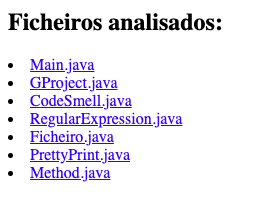
\includegraphics[scale=0.5]{images/indice-ficheiros.png}
    \caption{Índice dos ficheiros analisados.}
    \label{img:indice-ficheiros}
\end{figure}

De seguida, para cada ficheiro, são listadas as várias normas possíveis, tal como se pode verificar na figura \ref{img:indice-normas}.

\begin{figure}[H]
    \centering
    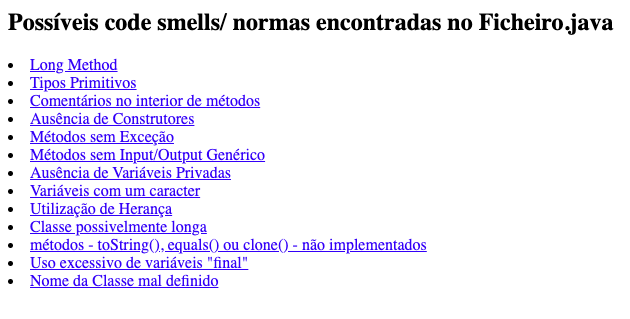
\includegraphics[scale=0.5]{images/indice-normas.png}
    \caption{Índice das normas possíveis no Ficheiro.java.}
    \label{img:indice-normas}
\end{figure}

Por fim, para cada norma listada, apresenta-se uma página com a informação adequada sobre a mesma, de seguida apresentam-se alguns exemplos de normas.

\begin{figure}[H]
    \centering
    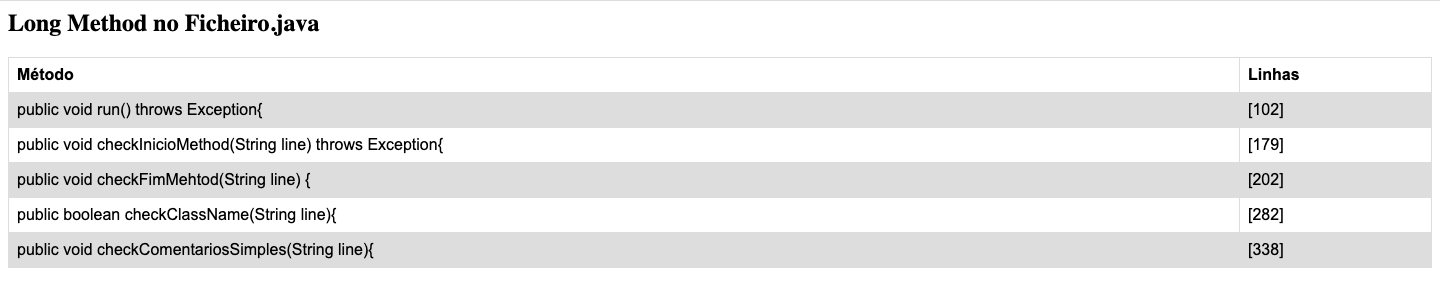
\includegraphics[scale=0.30]{images/n1.png}
    \caption{Informação sobre a norma Long Method.}
    \label{img:n1}
\end{figure}

\begin{figure}[H]
    \centering
    
\includegraphics[scale=0.5]{images/n2.png}
    \caption{Informação sobre a norma da existência de determinados métodos, tais como o toString, equals e clone.}
    \label{img:n1}
\end{figure}

\begin{figure}[H]
    \centering
    
\includegraphics[scale=0.5]{images/n4.png}
    \caption{Informação sobre a norma da ausência de variáveis privadas.}
    \label{img:n1}
\end{figure}

\begin{figure}[H]
    \centering
    
\includegraphics[scale=0.5]{images/n5.png}
    \caption{Informação sobre a norma da ausência de Construtores.}
    \label{img:n1}
\end{figure}

\begin{figure}[H]
    \centering
    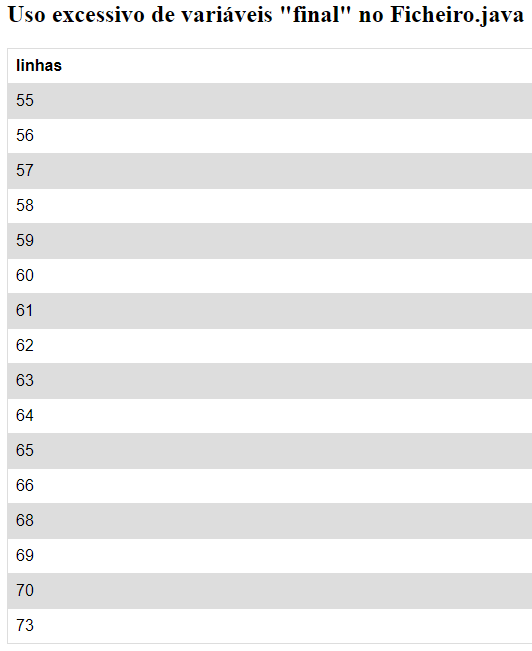
\includegraphics[scale=0.75]{images/manyFinals.PNG}
    \caption{Informação sobre a norma do uso excessivo de variáveis final.}
    \label{img:n1}
\end{figure}

\begin{figure}[H]
    \centering
    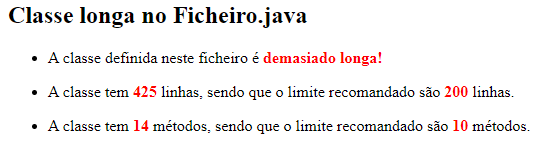
\includegraphics[scale=0.75]{images/large-class.PNG}
    \caption{Informação sobre a norma de classes grandes.}
    \label{img:n1}
\end{figure}
\chapter{Conclusão}

\par A criação deste sistema de análise estática de normas de codificação permitiu avaliar a qualidade de outros sistemas de software segundo as normas implementadas.
\par Efectivamente, o desenvolvimento deste trabalho consistiu numa divisão de tarefas pelos elementos do grupo de modo a, posteriormente, proceder a uma integração dos vários componentes já desenvolvidos. Este processo foi repetido várias vezes até se obter o produto final.
\par Posto isto, foram surgindo algumas dificuldades durante o desenvolvimento desta ferramenta. A titulo de exemplo tem-se a criação da expressão regular que deteta as declarações dos métodos usado no LongMethod, que foi depois reaproveitada para outros code smells específicos.
\par Finalmente, aquando da finalização do projecto, a ferramenta criada corresponde às expectativas inicialmente estabelecidas pelo que foi atingido um nível de satisfação aceitável. Para além disso, este projecto permitiu ao grupo de trabalho consolidar os conhecimentos sobre testes de software relativos a ferramentas de análise estática.
\begin{thebibliography}{9}
\bibitem{sourcemaking}
Source Making, \\
\texttt{https://sourcemaking.com/refactoring/smells}

\bibitem{Regex 101}
Regex 101, \\
\texttt{https://regex101.com/}

\bibitem{Stackoverflow}
Stackoverflow, \\
\texttt{https://stackoverflow.com/}

\end{thebibliography}

\newpage

\end{document}
